\chapter{Redes en Docker}
Con Docker podemos crear una gran cantidad de contenedores diferentes que se ejecuten de manera simultánea. Es lógico que a la hora de crear un sistema nos interese comunicar los contenedores entre ellos para que puedan transmitirse información. Como vamos a construir un sistema de paso mensajes entre contenedores con ROS (cómo usaremos ROS lo veremos en el siguiente capítulo) necesitamos crear una red entre esos contenedores. Para ello, en este capítulo se explicaran diferentes conceptos sobre configuración de redes en Docker. Por una parte se explican cosas básicas sobre redes con Docker y por otra parte herramientas más complejas que provee Docker (como \emph{ntework} o \emph{swarm}) para crear redes con topologías más complejas o redes multihost.

	\section{Redes básicas en Docker}

		\subsection{\textit{docker0}}
		Lo primero que hay que saber es que al iniciarse Docker, por defecto, se crea en el anfitrión (host) una interfaz virtual que tiene como nombre \textbf{\emph{docker0}} \cite{docker-network-advanced}. Docker coge de manera aleatoria una dirección IP y una subred de rango privado y se la asigna a \emph{docker0}. Las direcciones MAC de los contenedores se asignan usando la dirección IP de canda contenedor, para evitar de esta manera colisiones ARP.
		
		Lo que hace especial a \emph{docker0}, es que no solo es una interfaz, sino que es un puente Ethernet virtual que redirige automáticamente los paquetes entre cualquier otra interfaz que esté conectada a él. De esta manera se pueden comunicar tanto los contenedores entre ellos como con el host.
		
		Además desde un contenedor también se puede acceder a internet. En el capítulo anterior lanzamos contenedores que se creaban mediante los Dockerfiles que se obtenían del Docker Hub, que es un servidor web que se encuentra en internet. 
		
		Sin embargo, \textbf{no} podemos acceder a los contenedores desde fuera, desde internet. Por defecto está 
		establecido así, principalmente por temas de seguridad, aunque obviamente se puede cambiar.
		
		\subsection{Prueba de conexión entre contenedores}
		Si todos los contenedores que creamos se encuentran en una misma subred, podemos comunicarnos entre ellos simplemente con sus direcciones IP privadas o sus nombres de red. Vamos a hacer varias pruebas para comprobar que los contenedores se comunican bien entre ellos.
		
			\subsubsection{\textit{ping}}
			La forma más sencilla para probar la comunicación entre dos sistemas es el uso de la herramienta \emph{ping} de linux.
			
			Vamos a lanzar por una parte dos contenedores Docker en dos terminales separadas. Para esta prueba usaremos la misma imagen que vamos a usar para crear nuestro sistema, que es la imagen \emph{osrf/ros:indigo-desktop}, a la que previamente hemos hecho un \emph{pull} para tenerla generada, ya que ocupa alrededor de 1,6 GB. Creamos los contenedores de la siguiente manera.
			
			\begin{lstlisting}[style=consola]
$ docker run -it osrf/ros:indigo-desktop /bin/bash
			\end{lstlisting}
			
			Desde fuera comprobamos que tenemos los contenedores en ejecución.
			
			\begin{lstlisting}[style=consola,numbers=left]
$ docker ps
CONTAINER ID        IMAGE                     COMMAND                  CREATED             STATUS              PORTS               NAMES
829a49bb2cfa        osrf/ros:indigo-desktop   "/ros_entrypoint.sh /"   6 seconds ago       Up 6 seconds                            compassionate_mccarthy
2f3c19da0cb8        osrf/ros:indigo-desktop   "/ros_entrypoint.sh /"   16 seconds ago      Up 16 seconds                           grave_mahavira
			\end{lstlisting}
			
			Podemos obtener la dirección IP de un contenedor tanto desde fuera como desde dentro de Docker. En este caso lo haremos desde fuera mediante el \emph{inspect} de Docker.
			
			\begin{lstlisting}[style=consola,numbers=left]
$ docker inspect --format='{{.NetworkSettings.IPAddress}}' compassionate_mccarthy
172.17.0.5
$ docker inspect --format='{{.NetworkSettings.IPAddress}}' grave_mahavira
172.17.0.4
			\end{lstlisting}
			
			Ya tenemos las direcciones IP privadas que genera \emph{docker0} para los dos contenedores. Ahora probamos a hacer un ping desde un contenedor a otro. Desde el contenedor \textit{grave\_mahavira} con IP 172.17.0.4 al contenedor \textit{compassionate\_mccarthy} con IP 172.17.0.5 se haría así.
			
			\begin{lstlisting}[style=consola,numbers=left]
root@2f3c19da0cb8:/# ping 172.17.0.5
PING 172.17.0.5 (172.17.0.5) 56(84) bytes of data.
64 bytes from 172.17.0.5: icmp_seq=1 ttl=64 time=0.085 ms
64 bytes from 172.17.0.5: icmp_seq=2 ttl=64 time=0.058 ms
64 bytes from 172.17.0.5: icmp_seq=3 ttl=64 time=0.061 ms
64 bytes from 172.17.0.5: icmp_seq=4 ttl=64 time=0.060 ms
64 bytes from 172.17.0.5: icmp_seq=5 ttl=64 time=0.106 ms
64 bytes from 172.17.0.5: icmp_seq=6 ttl=64 time=0.135 ms
^C
--- 172.17.0.5 ping statistics ---
6 packets transmitted, 6 received, 0% packet loss, time 4997ms
rtt min/avg/max/mdev = 0.058/0.084/0.135/0.028 ms
			\end{lstlisting}
			
			Se puede hacer exactamente lo mismo con los nombres de los contenedores docker ya que esto son los nombres que se le dan en la red \emph{docker0} a la que están conectados. En este caso haremos un ping desde \textit{compassionate\_mccarthy} a \textit{grave\_mahavira} usando para ello el nombre del contenedor.
			
			\begin{lstlisting}[style=consola,numbers=left]
root@829a49bb2cfa:/# ping grave_mahavira
PING grave_mahavira (172.17.0.4) 56(84) bytes of data.
64 bytes from grave_mahavira.bridge (172.17.0.4): icmp_seq=1 ttl=64 time=0.087 ms
64 bytes from grave_mahavira.bridge (172.17.0.4): icmp_seq=2 ttl=64 time=0.066 ms
64 bytes from grave_mahavira.bridge (172.17.0.4): icmp_seq=3 ttl=64 time=0.066 ms
64 bytes from grave_mahavira.bridge (172.17.0.4): icmp_seq=4 ttl=64 time=0.067 ms
64 bytes from grave_mahavira.bridge (172.17.0.4): icmp_seq=5 ttl=64 time=0.066 ms
64 bytes from grave_mahavira.bridge (172.17.0.4): icmp_seq=6 ttl=64 time=0.064 ms
^C
--- grave_mahavira ping statistics ---
6 packets transmitted, 6 received, 0% packet loss, time 5001ms
rtt min/avg/max/mdev = 0.064/0.069/0.087/0.010 ms
			\end{lstlisting}
			
			Debido a esto, los nombres que se usan en los contendores deben ser \textbf{únicos}. Debemos tenerlo en cuanta a la hora de renombrar los contenedores. Tampoco podemos cambiar el nombre de un  contenedor durante su ejecucíon, solo podremos nombrarlo al lanzarlo.
			
			\subsubsection{\textit{netcat}}
			Otra forma de probar conexiones algo más versátil es el uso de \emph{netcat}. Netcat permite probar conexiones con cualquier tipo de puerto. Para probar que podemos usar cualquier puerto de los que no están predefinidos, vamos a usar la herramienta usando un puerto cualquiera de los que tenemos disponibles. En este caso lo haremos usando el puerto 1234. Para probarlo haremos lo siguiente.
			
			\begin{enumerate}
				\item Ejecutaremos en uno de los contenedores (da igual cual, la comunicación que se establecerá será bidireccional) netcat en modo escucha. En este caso lo haremos en \textit{grave\_mahavira}.
					\begin{lstlisting}[style=consola]
root@2f3c19da0cb8:/# netcat -l 1234

					\end{lstlisting}
				\item Desde el otro contenedor (\textit{compassionate\_mccarthy}) nos intentaremos conectar al primero.
					\begin{lstlisting}[style=consola]
root@829a49bb2cfa:/# netcat grave_mahavira 1234

					\end{lstlisting}			
				\item Si todo ha salido bien, podremos escribir desde cualquiera de los dos terminales y aparecerá lo introducido en el otro.
				\begin{enumerate}
					\item Escribimos en \textit{grave\_mahavira}.
					\begin{lstlisting}[style=consola]
root@2f3c19da0cb8:/# netcat -l 1234
Hola!

					\end{lstlisting}
					\begin{lstlisting}[style=consola]
root@829a49bb2cfa:/# netcat grave_mahavira 1234
Hola!

					\end{lstlisting}	
					\item Y ahora en \textit{compassionate\_mccarthy}
					\begin{lstlisting}[style=consola]
root@2f3c19da0cb8:/# netcat -l 1234
Hola!
Hola de nuevo!				
					
					\end{lstlisting}
					\begin{lstlisting}[style=consola]
root@829a49bb2cfa:/# netcat grave_mahavira 1234
Hola!
Hola de nuevo!
	
					\end{lstlisting}
				\end{enumerate}
			\end{enumerate}
		
		\subsection{Links entre contenedores}
		Como hemos visto, a causa de tener los contenedores dentro de una red privada, comunicarlos entre ellos es algo trivial. El problema de transmitir información de esta manera es que el interfaz \emph{docker0} se usa para \textbf{todos} los contenedores que estén en ejecución en ese host. Si queremos realizar una comunicación privada entre dos contenedores, que sea invisible para el resto de contenedores, debemos usar el mecanismo que provee Docker, el linkado de contenedores \cite{docker-network-linking}.
		
		Docker provee también un sistema para mapear puertos entre dos contenedores, aunque el mejor sistema que podemos usar para conectar contendores el el linkado, ya que abstrae todo el sistema de puertos, y crea un puente virtual que permite una comunicación segura entre los contenedores.
		
		Para usar el sistema de links de Docker, debemos usar el flag \textbf{--link} a la hora de lanzar el contenedor. Primero vamos a crear un contenedor al que llamaremos ros1.
		
		\begin{lstlisting}[style=consola]
$ docker run -it --name ros1 osrf/ros:indigo-desktop /bin/bash
		\end{lstlisting}
		
		A continuación vamos a crear otro contenedor, al que llamaremos \emph{ros2}, que este linkado a \emph{ros1}.
		
		\begin{lstlisting}[style=consola]
$ docker run -it --name ros2 --link ros1 osrf/ros:indigo-desktop /bin/bash
		\end{lstlisting}
		
		Ahora desde fuera de los contenedores, miramos los links que tiene \emph{ros2} mediante \emph{inspect}.
		
		\begin{lstlisting}[style=consola,numbers=left]
$ docker inspect -f "{{ .HostConfig.Links }}" ros2
[/ros1:/ros2/ros1]
		\end{lstlisting}
		
		Ahora desde \emph{ros2} podemos acceder a la información de \emph{ros1}.
		
		Para lograr este enlace Docker usa dos sistemas diferentes:
		
		\begin{itemize}
			\item Variables de entorno
			\item Actualizar el fichero \emph{/etc/hosts}
		\end{itemize}
		
		Todo esto lo realiza de manera automática a la hora de enlazar dos contenedores.
	
	\section{Redes avanzadas con Docker}
	
		\subsection{\textit{network} de Docker}
		En la verión 1.9 de Docker (la que se usa en este documento) se implementó una nueva funcionalidad que llevaba gestándose desde que salió la versión 1.7. Esta nueva funcionalidad permite crear redes con diferentes topologías de una manera sencilla, abstrayendo de configuraciones, al igual que los links de Docker. A diferencia de los links de Docker, que está más orientados a conectar directamente contenedores, esta nueva funcionalidad permite crear redes virtuales enteras.
		
		La forma de trabajar con esta funcionalidad es mediante el uso del comando \textit{\emph{network}}.
		
		\begin{lstlisting}[style=consola]
$ docker network --help

Usage:	docker network [OPTIONS] COMMAND [OPTIONS]

Commands:
disconnect               Disconnect container from a network
inspect                  Display detailed network information
ls                       List all networks
rm                       Remove a network
create                   Create a network
connect                  Connect container to a network

Run 'docker network COMMAND --help' for more information on a command.

--help=false       Print usage
		\end{lstlisting}
		
			\subsubsection{Prueba de \textit{network}}
			Vamos a crear una red a la que posteriormente vamos a unir dos contedores cualquiera (Ubuntu mismo) y haremos pruebas como las anteriores para comprobar que funciona la red que hemos creado.
			
			\begin{enumerate}
				\item Creamos la red.
				\begin{lstlisting}[style=consola]
$ docker network create red-prueba
6a9b1bceb5e8033744d4220da1c2e144aea9543bdea0804af0261d973b7bd57e
				\end{lstlisting}
			
				\item Creamos dos contenedores Docker.
				\begin{lstlisting}[style=consola]
$ docker run -it --name ubuntu1 ubuntu /bin/bash
root@f5225f49f6a9:/# 
				\end{lstlisting}
				\begin{lstlisting}[style=consola]
$ docker run -it --name ubuntu2 ubuntu /bin/bash
root@969d7f0c6a5b:/# 
				\end{lstlisting}
				
				\item Añadimos desde el host los dos contendores Docker a la red. Esto se puede hacer de dos maneras. Se puede indicar la red a la que conectarse en el momento en el que creamos el contenedor o se puede hacer después mediante el subcomando \emph{connect} que tiene \emph{network}. Lo haremos de la segunda manera ya que nos permite usar contenedores ya creados.
				\begin{lstlisting}[style=consola]
$ docker network connect red-prueba ubuntu1
$ docker network connect red-prueba ubuntu2 
				\end{lstlisting}
				
				\item Probamos la conexión desde los contenedores
				\begin{enumerate}
					\item Hacemos \textit{ping} entre los contenedores.
					\begin{lstlisting}[style=consola,numbers=left]
root@f5225f49f6a9:/# ping ubuntu2
PING ubuntu2 (172.19.0.3) 56(84) bytes of data.
64 bytes from ubuntu2 (172.19.0.3): icmp_seq=1 ttl=64 time=0.144 ms
64 bytes from ubuntu2 (172.19.0.3): icmp_seq=2 ttl=64 time=0.066 ms
64 bytes from ubuntu2 (172.19.0.3): icmp_seq=3 ttl=64 time=0.066 ms
^C
--- ubuntu2 ping statistics ---
3 packets transmitted, 3 received, 0% packet loss, time 1998ms
rtt min/avg/max/mdev = 0.066/0.092/0.144/0.036 ms
					\end{lstlisting}
					\begin{lstlisting}[style=consola,numbers=left]
root@969d7f0c6a5b:/# ping ubuntu1
PING ubuntu1 (172.19.0.2) 56(84) bytes of data.
64 bytes from ubuntu1 (172.19.0.2): icmp_seq=1 ttl=64 time=0.062 ms
64 bytes from ubuntu1 (172.19.0.2): icmp_seq=2 ttl=64 time=0.077 ms
64 bytes from ubuntu1 (172.19.0.2): icmp_seq=3 ttl=64 time=0.060 ms
64 bytes from ubuntu1 (172.19.0.2): icmp_seq=4 ttl=64 time=0.067 ms
^C
--- ubuntu1 ping statistics ---
4 packets transmitted, 4 received, 0% packet loss, time 2999ms
rtt min/avg/max/mdev = 0.060/0.066/0.077/0.010 ms
					\end{lstlisting}
					
					\item Usamos \textit{netcat} con un puerto mayor que el 1024.
					\begin{lstlisting}[style=consola]
root@f5225f49f6a9:/# netcat -l 1234
Hola
que tal?
					\end{lstlisting}
					\begin{lstlisting}[style=consola]
root@969d7f0c6a5b:/# netcat ubuntu1 1234
Hola
que tal?
					\end{lstlisting}
				\end{enumerate}
			\end{enumerate}
			
		\subsection{Redes Multi-Host}
		Para crear redes Multi-Host con Docker lo mejor es usar Docker Swarm. Docker Swarm es una herramienta que provee Docker que sirve para crear clusters de contenedores Docker. Para crear redes Multi-Host con esta herramienta necesitamos instalar en el host lo siguiente:
		
		\begin{enumerate}
			\item \textbf{VirtualBox}.
			\item \textbf{Docker Machine}. Docker Machine es un software proporcionado por los creadores de Docker que nos permite crear diferentes hosts en un mismo sistema. \cite{docker-machine} Permite lanzar demonios del proceso \textit{docker} independientes entre sí.
		\end{enumerate}
		
		En caso de usar Docker desde OS X o desde Windows deberíamos tener ya VirtualBox instalado.
		
			\subsubsection{Instalación de Swarm}
			Para instalar las herramientas necesarias (en un sistema GNU-Linux) haremos lo siguiente:
			\begin{itemize}
				\item Instalamos VirtualBox desde el gestor de paquetes. Para Debian y derivados usamos apt-get.
				\begin{lstlisting}[style=consola]
$ sudo apt-get install virtualbox
				\end{lstlisting}
				\item Para instalar Docker Machine hay que seguir los siguientes pasos: \cite{docker-machine-install}
				\begin{enumerate}
					\item Instalamos Docker Machine con el siguiente comando (instala la versión  v0.5.0, que al escribir este documento es la última versión).
					\begin{lstlisting}[style=consola,numbers=left]
$ curl -L https://github.com/docker/machine/releases/download/v0.5.0/docker-machine_linux-amd64.zip >machine.zip && \
unzip machine.zip && \
rm machine.zip && \
sudo mv docker-machine* /usr/local/bin
					\end{lstlisting}
					\item Comprobamos que se ha instalado correctamente mediante el siguiente comando.
					\begin{lstlisting}[style=consola,numbers=left]
$ docker-machine -v
docker-machine version 0.5.0 (04cfa58)
					\end{lstlisting}
				\end{enumerate}
				\item Para instalar Swarm simplemente hacemos un pull de la imagen de Swarm mediante Docker, la cual posteriormente instanciaremos y le añadiremos nodos con sus respectivos contenedores dentro de ellos.
				\begin{lstlisting}[style=consola]
$ docker pull swarm
				\end{lstlisting}
			\end{itemize}
		
			\subsubsection{Creación de un Swarm}
			Hay que distinguir tres conceptos para comprender el funcionamiento de Docker Swarm. Son los siguientes:
			\begin{itemize}
				\item \textbf{Docker Node (Nodo Docker)}: una máquina ejecutando el demonio de Docker (la cual puede tener diferentes contenedores)
				\item \textbf{Swarm Host (Anfitrión Swarm)}: Una máquina ejecutando el demonio de Swarm
				\item \textbf{Swarm (Enjambre)}: Una serie de Nodos Docker
			\end{itemize}
			
			La creación del Swarm se llevara a cabo desde el host Windows y no desde la VM con GNU/Linux. Esto es debido a que es necesario que el SO soporte tecnología de virtualización, y hacer que una VM soporte virtualizacián para crear más VMs dentro de ella es un proceso redundate e innecesario.
			
			De todas maneras el proceso de creación del Swarm es análogo, y en el caso de Windows, Docker Machine ya viene instalado como dependencia del Docker Toolbox, que es la herramienta mediante la que se instala todo el entorno de Docker en sistemas operativos Windows.
			
			Docker Toolbox se puede obtener para plataformas Mac y Windows desde el siguiente enlace: \url{https://www.docker.com/docker-toolbox}.
			
			Los pasos para crear un Swarm son los siguientes: \cite{docker-swarm-and-machine}
			\begin{enumerate}
				\item Vemos los host Docker de nuestro sistema.
				\begin{lstlisting}[style=consola,numbers=left]
$ docker-machine ls
NAME      ACTIVE   URL          STATE     URL                         SWARM   DOCKER   ERRORS
default   *        virtualbox   Running   tcp://192.168.99.100:2376           v1.9.1
				\end{lstlisting}
				En este caso vemos uno llamado \textit{default}. Ese es el que usa Docker para ejecutar Docker en Windows. En caso de usar Docker desde GNU/Linux ese host no se mostraría.
			
				\item Creamos una máquina virtual en VirtualBox llamada \textit{local}.
				\begin{lstlisting}[style=consola,numbers=left]
$ docker-machine create -d virtualbox local
Running pre-create checks...
Creating machine...
(local) Copying C:\Users\ander\.docker\machine\cache\boot2docker.iso to C:\Users\ander\.docker\machine\machines\local\boot2docker.iso...
(local) Creating VirtualBox VM...
(local) Creating SSH key...
(local) Starting the VM...
(local) Waiting for an IP...
Waiting for machine to be running, this may take a few minutes...
Machine is running, waiting for SSH to be available...
Detecting operating system of created instance...
Detecting the provisioner...
Provisioning with boot2docker...
Copying certs to the local machine directory...
Copying certs to the remote machine...
Setting Docker configuration on the remote daemon...
Checking connection to Docker...
Docker is up and running!
To see how to connect Docker to this machine, run: C:\Program Files\Docker Toolbox\docker-machine.exe env local
				\end{lstlisting}

				\item Cargamos la configuración de la maquina en la shell.
				\begin{lstlisting}[style=consola,numbers=left]
$ eval "$(docker-machine env local)"
				\end{lstlisting}
			
				\item Generamos un \textit{discovery token} mediante la imagen de Swarm de Docker. Este token nos servira para gestionar el Swarm más adelante.
			
				El comando de abajo ejecuta el comando \textit{create} de Swarm en un contenedor. Descargará la imagen automáticamente en caso de no tenerla, como de costumbre.
				
				\begin{lstlisting}[style=consola,numbers=left]
$ docker run swarm create
Unable to find image 'swarm:latest' locally
latest: Pulling from swarm
d681c900c6e3: Pull complete
188de6f24f3f: Pull complete
90b2ffb8d338: Pull complete
237af4efea94: Pull complete
3b3fc6f62107: Pull complete
7e6c9135b308: Pull complete
986340ab62f0: Pull complete
a9975e2cc0a3: Pull complete
Digest: sha256:c21fd414b0488637b1f05f13a59b032a3f9da5d818d31da1a4ca98a84c0c781b
Status: Downloaded newer image for swarm:latest
dc60acd12fc3a6b14754abef91501be2
				\end{lstlisting}
			
				\item Guarmamos el token que nos devuelve ya que lo necesitaremos para más adelante. En nuetro caso es dc60acd12fc3a6b14754abef91501be2.
				
				Si abrimos VirtualBox podremos observar que tenemos dos máquinas de tipo GNU/Linux, la que acabamos de crear y la que usa Docker para ejecutarse.
				
				\begin{figure}[H] % Con el parámetro H la imagens se muestra justo en el sitio en el que se ha definido
					\centering
					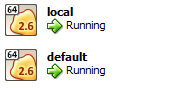
\includegraphics{VBoxSwarm}
					\caption{Imágenes GNU/Linux creadas}
					\label{fig:VBoxSwarm}
				\end{figure}
			
			\end{enumerate}
			
			\subsubsection{Lanzar el \textit{Swarm manager}}
			Para crear un Swarm, primero es necesario crear una maquina llamada \textit{Swarm manager}. El \textit{Swarm manager} dirige y maneja todos los contenedores del clúster, es decir, todos los Nodos Docker.
			
			Despues de crear el \textit{Swarm manager}, hay que crear una serie de Nodos Docker, que son los que se encargaran de ejecutar instancias de Docker y de manejar contenedores.
			
			A continuación vamos a crear un \textit{Swarm manager} y dos Nodos Docker. Para ello usamos el comando \textit{create} de Docker Machine, usando el token anotado anteriormente y diferentes flags que veremos a continuación.
			
			\begin{enumerate}
				\item Creamos un Swarm manager bajo VirtualBox.
				\begin{lstlisting}[style=consola,numbers=left]
$ docker-machine create -d virtualbox --swarm --swarm-master --swarm-discovery token://dc60acd12fc3a6b
14754abef91501be2 swarm-master
Running pre-create checks...
Creating machine...
(swarm-master) Copying C:\Users\ander\.docker\machine\cache\boot2docker.iso to C:\Users\ander\.docker\machine\machines\swarm-master\boot2docker.iso...
(swarm-master) Creating VirtualBox VM...
(swarm-master) Creating SSH key...
(swarm-master) Starting the VM...
(swarm-master) Waiting for an IP...
Waiting for machine to be running, this may take a few minutes...
Machine is running, waiting for SSH to be available...
Detecting operating system of created instance...
Detecting the provisioner...
Provisioning with boot2docker...
Copying certs to the local machine directory...
Copying certs to the remote machine...
Setting Docker configuration on the remote daemon...
Configuring swarm...
Checking connection to Docker...
Docker is up and running!
To see how to connect Docker to this machine, run: C:\Program Files\Docker Toolbox\docker-machine.exe env swarm-master
				\end{lstlisting}
				
				Para indicar que es el Swarm manager usamos el flag \textit{--swarm-master}.
				
				\item Creamos un nodo Swarm. Lo llamaremos \textit{swarm-agent-00}.
				\begin{lstlisting}[style=consola,numbers=left]
$ docker-machine create -d virtualbox --swarm --swarm-discovery token://dc60acd12fc3a6b14754abef91501b
e2 swarm-agent-00
Running pre-create checks...
Creating machine...
(swarm-agent-00) Copying C:\Users\ander\.docker\machine\cache\boot2docker.iso to C:\Users\ander\.docker\machine\machines\swarm-agent-00\boot2docker.iso...
(swarm-agent-00) Creating VirtualBox VM...
(swarm-agent-00) Creating SSH key...
(swarm-agent-00) Starting the VM...
(swarm-agent-00) Waiting for an IP...
Waiting for machine to be running, this may take a few minutes...
Machine is running, waiting for SSH to be available...
Detecting operating system of created instance...
Detecting the provisioner...
Provisioning with boot2docker...
Copying certs to the local machine directory...
Copying certs to the remote machine...
Setting Docker configuration on the remote daemon...
Configuring swarm...
Checking connection to Docker...
Docker is up and running!
To see how to connect Docker to this machine, run: C:\Program Files\Docker Toolbox\docker-machine.exe env swarm-agent-00
				\end{lstlisting}

				\item Creamos otro nodo Swarm. Lo llamaremos \textit{swarm-agent-01}.
				\begin{lstlisting}[style=consola,numbers=left]
$ docker-machine create -d virtualbox --swarm --swarm-discovery token://dc60acd12fc3a6b14754abef91501b
e2 swarm-agent-01
Running pre-create checks...
Creating machine...
(swarm-agent-01) Copying C:\Users\ander\.docker\machine\cache\boot2docker.iso to C:\Users\ander\.docker\machine\machines\swarm-agent-01\boot2docker.iso...
(swarm-agent-01) Creating VirtualBox VM...
(swarm-agent-01) Creating SSH key...
(swarm-agent-01) Starting the VM...
(swarm-agent-01) Waiting for an IP...
Waiting for machine to be running, this may take a few minutes...
Machine is running, waiting for SSH to be available...
Detecting operating system of created instance...
Detecting the provisioner...
Provisioning with boot2docker...
Copying certs to the local machine directory...
Copying certs to the remote machine...
Setting Docker configuration on the remote daemon...
Configuring swarm...
Checking connection to Docker...
Docker is up and running!
To see how to connect Docker to this machine, run: C:\Program Files\Docker Toolbox\docker-machine.exe env swarm-agent-01
				\end{lstlisting}
	
				\item Si miramos de nuevo en VirtualBox, veremos que tenemos las 3 nuevas máquinas que acabamos de crear junto a las dos que teníamos anteriormente.
				
				\begin{figure}[H] % Con el parámetro H la imagens se muestra justo en el sitio en el que se ha definido
					\centering
					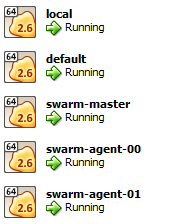
\includegraphics{VBoxSwarm2}
					\caption{Imágenes GNU/Linux creadas para el Swarm}
					\label{fig:VBoxSwarm2}
				\end{figure}
				
			\end{enumerate}
			
			\subsubsection{Configurar el Swarm y lanzar contenedores}
			
			\begin{enumerate}
				\item Apuntamos nuestro entorno Docker a la máquina que está ejecutando el Swarm master.
				\begin{lstlisting}[style=consola,numbers=left]
$ eval $(docker-machine env --swarm swarm-master)
				\end{lstlisting}
				
				\item Obtenemos informacion sobre el Swarm creado mediante el comando \textit{info} de Docker.
				\begin{lstlisting}[style=consola,numbers=left]
$ docker info
Containers: 4
Images: 3
Role: primary
Strategy: spread
Filters: health, port, dependency, affinity, constraint
Nodes: 3
 swarm-agent-00: 192.168.99.103:2376
   Status: Healthy
   Containers: 1
   Reserved CPUs: 0 / 1
   Reserved Memory: 0 B / 1.021 GiB
   Labels: executiondriver=native-0.2, kernelversion=4.1.13-boot2docker, operatingsystem=Boot2Docker 1.9.1 (TCL 6.4.1); master : cef800b - Fri Nov 20 19:33:59 UTC 2015, provider=virtualbox, storagedriver=aufs
 swarm-agent-01: 192.168.99.104:2376
   Status: Healthy
   Containers: 1
   Reserved CPUs: 0 / 1
   Reserved Memory: 0 B / 1.021 GiB
   Labels: executiondriver=native-0.2, kernelversion=4.1.13-boot2docker, operatingsystem=Boot2Docker 1.9.1 (TCL 6.4.1); master : cef800b - Fri Nov 20 19:33:59 UTC 2015, provider=virtualbox, storagedriver=aufs
 swarm-master: 192.168.99.102:2376
   Status: Healthy
   Containers: 2
   Reserved CPUs: 0 / 1
   Reserved Memory: 0 B / 1.021 GiB
   Labels: executiondriver=native-0.2, kernelversion=4.1.13-boot2docker, operatingsystem=Boot2Docker 1.9.1 (TCL 6.4.1); master : cef800b - Fri Nov 20 19:33:59 UTC 2015, provider=virtualbox, storagedriver=aufs
CPUs: 3
Total Memory: 3.064 GiB
Name: swarm-master
				\end{lstlisting}
				
				Se puede observar que tanto el manager como lon nodos tienen el puerto 2376 expuesto. Cuando se crea un Swarm se puede usar el puerto que se quiera, e incluso usar diferentes puertos para diferentes nodos. Cada nodo del Swarm ejecuta un gestor de contenedores Docker.
				
				En el caso del master, ejecuta tanto el gestor de contenedores como el Swarm manager. Esto no suele ser recomendable en entornos de producción.
				
				\item Consultamos las imágenes en ejecución en el Swarm.
				\begin{lstlisting}[style=consola,numbers=left]
$ docker ps -a
CONTAINER ID        IMAGE               COMMAND                  CREATED             STATUS              PORTS               NAMES
3f228154f8ff        swarm:latest        "/swarm join --advert"   20 minutes ago      Up 20 minutes                           swarm-agent-01/swarm-agent
e9df36929545        swarm:latest        "/swarm join --advert"   22 minutes ago      Up 22 minutes                           swarm-agent-00/swarm-agent
a18b76c0013d        swarm:latest        "/swarm join --advert"   27 minutes ago      Up 27 minutes                           swarm-master/swarm-agent
35fcf51df08a        swarm:latest        "/swarm manage --tlsv"   27 minutes ago      Up 27 minutes                           swarm-master/swarm-agent-master
				\end{lstlisting}
				
				\item Lanzamos una imagen en el Swarm. Vamos a usar la ya conocida \textit{hello-world}.
				\begin{lstlisting}[style=consola,numbers=left]
$ docker run hello-world

Hello from Docker.
This message shows that your installation appears to be working correctly.

To generate this message, Docker took the following steps:
1. The Docker client contacted the Docker daemon.
2. The Docker daemon pulled the "hello-world" image from the Docker Hub.
3. The Docker daemon created a new container from that image which runs the
executable that produces the output you are currently reading.
4. The Docker daemon streamed that output to the Docker client, which sent it
to your terminal.

To try something more ambitious, you can run an Ubuntu container with:
$ docker run -it ubuntu bash

Share images, automate workflows, and more with a free Docker Hub account:
https://hub.docker.com

For more examples and ideas, visit:
https://docs.docker.com/userguide/
				\end{lstlisting}
				
				\item Vamos a usar el comando \textit{ps} de Docker para ver en que nodo se ha ejecutado el contenedor.
				\begin{lstlisting}[style=consola,numbers=left]
$ docker ps -a
CONTAINER ID        IMAGE               NAMES
91a89b22a8b1        hello-world         swarm-agent-00/sleepy_perlman
3f228154f8ff        swarm:latest        swarm-agent-01/swarm-agent
e9df36929545        swarm:latest        swarm-agent-00/swarm-agent
a18b76c0013d        swarm:latest        swarm-master/swarm-agent
35fcf51df08a        swarm:latest        swarm-master/swarm-agent-master
				\end{lstlisting}
				
				Como se puede observar se ha ejecutado en el nodo \textit{swarm-agent-00}.
			\end{enumerate}
			
			Una vez visto el funcionamiento de Swarm y las redes Multi-Host en Docker, podemos complicar nuestro sistema tanto como queramos. Podemos lanzar diferentes nodos en diferentes sistemas separados dentro de una misma red o entre diferentes redes conectadas entre sí. En la documentación de Swarm \cite{docker-swarm} se puede encontrar más información al respecto.	
	
	\section{Configuración manual de redes}
	Aunque en este capítulo se han enseñado varios mecanismos que provee Docker para administrar redes de contenedores, también podemos configurar toda nuestra red de una manera más tradicional, mediante la modificación de archivos como \emph{/etc/hosts} o \emph{/etc/interfaces} en nuestros contenedores, el uso de \emph{Iptables}, configuración de DNS,... 
	
	Docker mediante estos mecanismos busca abstraer parte de la configuración para hacerla mas sencilla de cara al desarrollador o al administrador.
	
	Prácticamente cualquier aspecto relacionado con las redes se puede configurar en Docker mediante una serie de flags especiales a la hora de lanzar el servicio de Docker, por lo que no se pueden modificar mientras Docker esté en ejecución (no confundir con que un contenedor esté en ejecución). Algunos de esos comandos con flags especiales solo se pueden ejecutar con el servicio de Docker parado. Varios de los mas importantes son.
	
	\begin{lstlisting}[style=consola,numbers=left]
--default-gateway=IP_ADDRESS # Define la IP a la que se conectaran los contenedores de Docker al crearse, por defecto se usa la de docker0
--icc=true|false # Indica si se permite la comunicacion entre contenedores, por defecto true
--ipv6=true|false # Define si se usa IPv6, por defecto false
--ip-forward=true|false # Indica si esta activada la comunicacion entre los contenedores y el exterior, por defecto true
--iptables=true|false # Define si se perminte el uso de iptables (filtra direcciones y puertos, se usa como firewall en sistemas tipo UNIX)
	\end{lstlisting}
	
	En la documentación de Networking avanzado de Docker \cite{docker-network-advanced} se puede encontrar mucha más información de como hacer esto.
	